\documentclass[a4paper,twoside]{article}
\usepackage{graphicx, fullpage, float, verbatim,amsmath, subcaption, listings}

\title{Evolution of CO2e multipliers over time: the case of French Agriculture}
\author{Molly Bazilchuk & Mohamed Badr}
\date{\today}


\begin{document}
\maketitle
\vspace{3cm}
\bibliographystyle{abbrv}

\section{Introduction}

Globally, food production is responsible for around one-quarter of the world's greenhouse gas emissions, while agriculture, forestry and land-use change account for around 18\%. Reducing agricultural emissions will therefore be key in limiting the extent of climate change. In terms of agricultural, France is the largest producer in Europe and is therefore an interest case for study when considering emissions intensity change over time. The French Ministry for Agriculture and Food stated in 2018 their goal to reduce emissions by 50\% by 2050 compared to 1990 levels. However, as is the case with the majority of government pledges, this deals with direct emissions rather than footprint or consumption-based emissions as is considered in input-output analysis. 

In this work, we perform an input-output analysis of the agricultural products of France. The multipliers in $kgCO_2e/Euro$ are considered in particular, in order to decouple changes in the production intensity from effects of the final demand. While many IO studies choose to aggregate products in input-output tables to more general categories, we have kept the original agricultural sectors to profit from the detail in the EXIOBASE data.

There are few comparable studies in the literature. Liu et al. looked at the change of pollutants and carbon emissions multipliers in China in the period 2007 - 2012, considering overall changes in the different sectors of the economy \cite{Liu2017}. Camanzi et al. consider agriculture in the EU in particular, and maintained product category resolution in their analysis, but considered the total emissions only rather than the multipliers \cite{Camanzi2017}. Schneider et al. considered the energy intensity of global agriculture and how it has evolved since the 1960's, but the analysis is based on broader economic data rather than input-output tables and so lacks sector evolution \cite{Schneider2009}.

\section{Methods and data}

\subsection{Database}

The analysis was performed using EXIOBASE 3, the multi-regional input-output database with high sectoral resolution (200 products) and most accurate environmental extensions \cite{Stadler2018}. The scope of our model system was the 15 primary agricultural products. There are also secondary agricultural products (e.g. "dairy products" as opposed to "cattle"), but as our focus was on the production itself we excluded these. Due to computational limitations, we studied every other year starting from the year 1996 and ending at the year 2022. The data was analysed using the Pymrio Python package; relevant code can be found in Appendix A.

\subsection{Multiplier calculation}

For an input-output system, a multiplier is a quantity that, when multiplied with the final demand, gives the total emissions of a pollutant or other quantity such as energy consumption, labor use, etc. Multipliers $M$ are derived by performing the firm balance for some amount of emissions $F$, where $Z$ is the inter-industry flow matrix describing intermediate demand flowing between industries, and $x$ is the total output vector.

\begin{equation}
F + M Z = M \hat{x}
\end{equation}

We can then rearrange and express as a function of the Leontief inverse $L$ for a system.

\begin{equation}
M = F \hat{x}^{-1} (I - A)^{-1} = f \hat{x} L
\end{equation}

This calculation is performed automatically by the Pymrio Python package.

\subsection{Impacts}

Impacts were aggregated into GHG emissions “(GWP100) | Problem oriented approach: baseline (CML, 2001) | GWP100 (IPCC, 2007)”. This is done through characterization, which allows us to gain a broader perspective of all the GHG related impacts per product. After a primary analysis we then normalise all the multiplier values on the base year of 1996. This allows the research to better understand the evolution of multiplier values within a given time frame.

\subsection{Inflation}

To adjust for inflation, we use the Food and Agriculture Organisation of the United Nations (FAOSTAT) data on inflation in the French agricultural sector in the relevant time frame. Given the absence of product specific inflation statistics, this was the most relevant inflation data available. We normalise all prices on the base year 2015 as per FAOSTAT. Given that FAOSTAT only provides inflation figures from the year 2000 we used the inflation rate for the year 2000 for the years 1996 and 1998. More so, the inflation rate for the year 2022 has not been released yet (for the relevant sectors), we therefore use the inflation rate of the previous year (2021).

\section{Results}

Fig. \ref{fig:rawmultipliers} shows the normalized evolution of the agricultural multipliers from the year 1996 - 2022 as obtained directly from the Pymrio calculation. We can see that animal production sectors such as cattle, animal products, raw milk and meat animals nec have by far with largest multipliers per euro sold. This again is for the production sectors, whereas EXIOBASE incorporates other product sectors for the final products as sold to consumers.

Based on the raw multipliers, it would appear that the trend is a decrease in multipliers over the time period considered. However, as we will see in the next figure, this is misleading.

\begin{figure}[H]
\centering
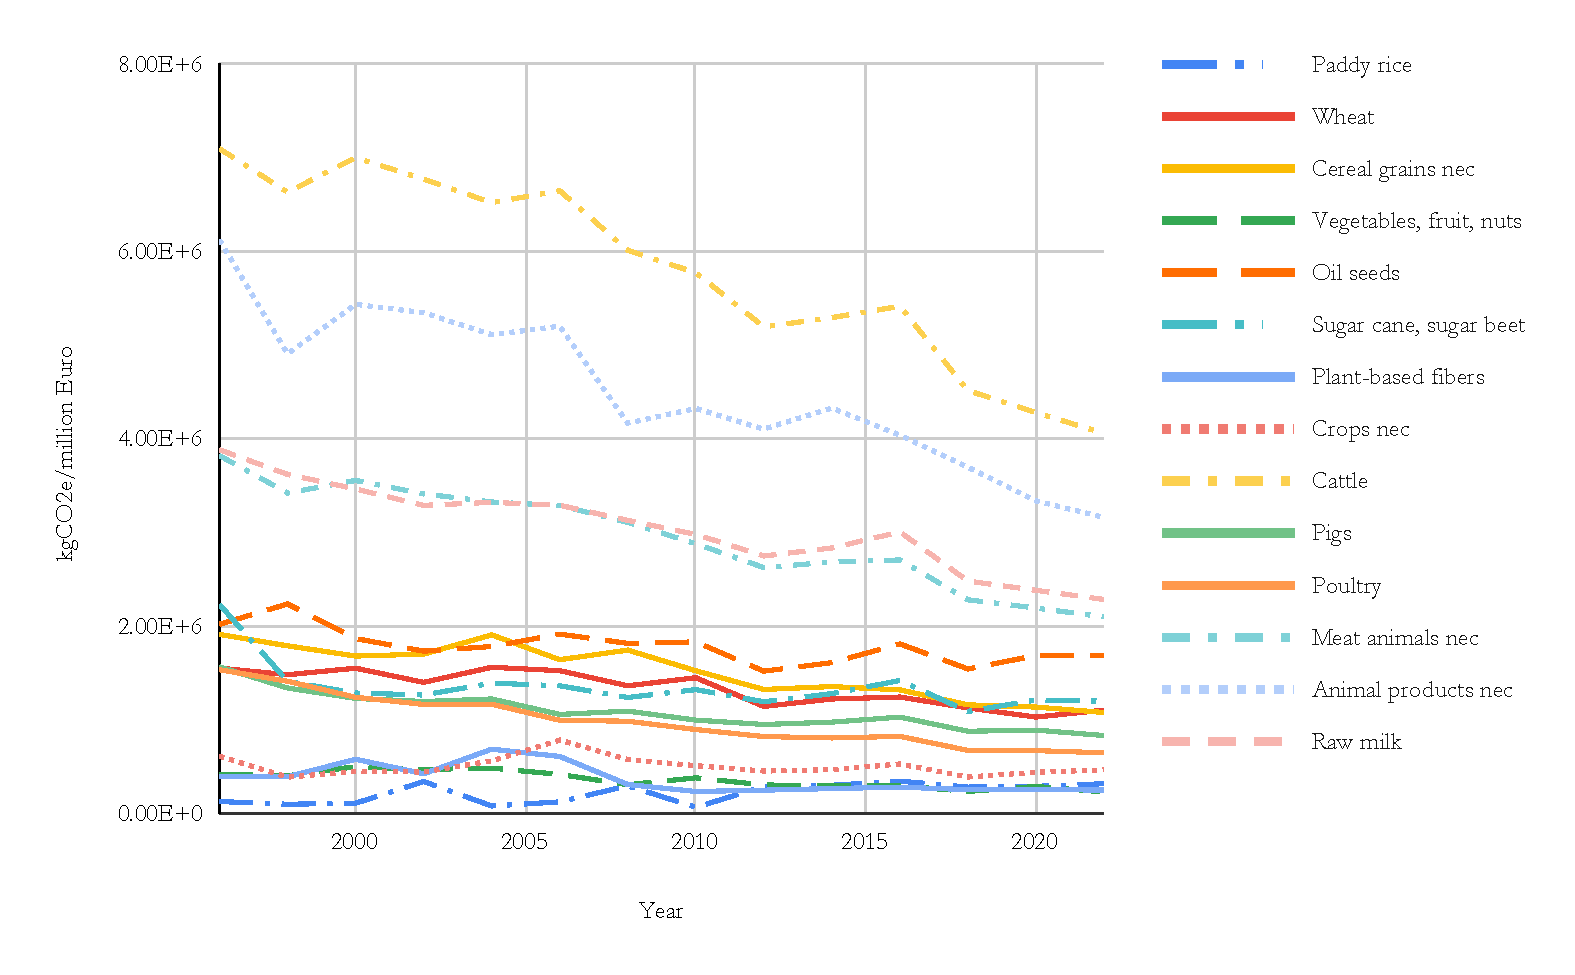
\includegraphics[width=0.9\textwidth]{raw_multipliers}
\caption{The multipliers per sector for French agriculture 1996 - 2022.}\label{fig:rawmultipliers} 
\end{figure}

Since multipliers are expressed in terms of currency, changes over time cannot be properly considered without taking into account the effects of inflation. The multipliers were therefore adjusted using the consumer price indices from FAOSTAT. Applying this index is a simplification, as inflation in certain sectors of agriculture might be larger than others. Furthermore the inflation indices are for end consumer prices whereas we are considering intermediate agricultural products. We consider it good enough for a first order estimate. The consumer price indices are given with a base year of 2015, such that the multipliers for earlier years are general lower that in Fig. \ref{fig:rawmultipliers} and later years increase.

Fig. \ref{fig:adjustedmultipliers} shows the inflation-adjusted multipliers for the agricultural sectors. The downward trend is now far less prominent. 

\begin{figure}[H]
\centering
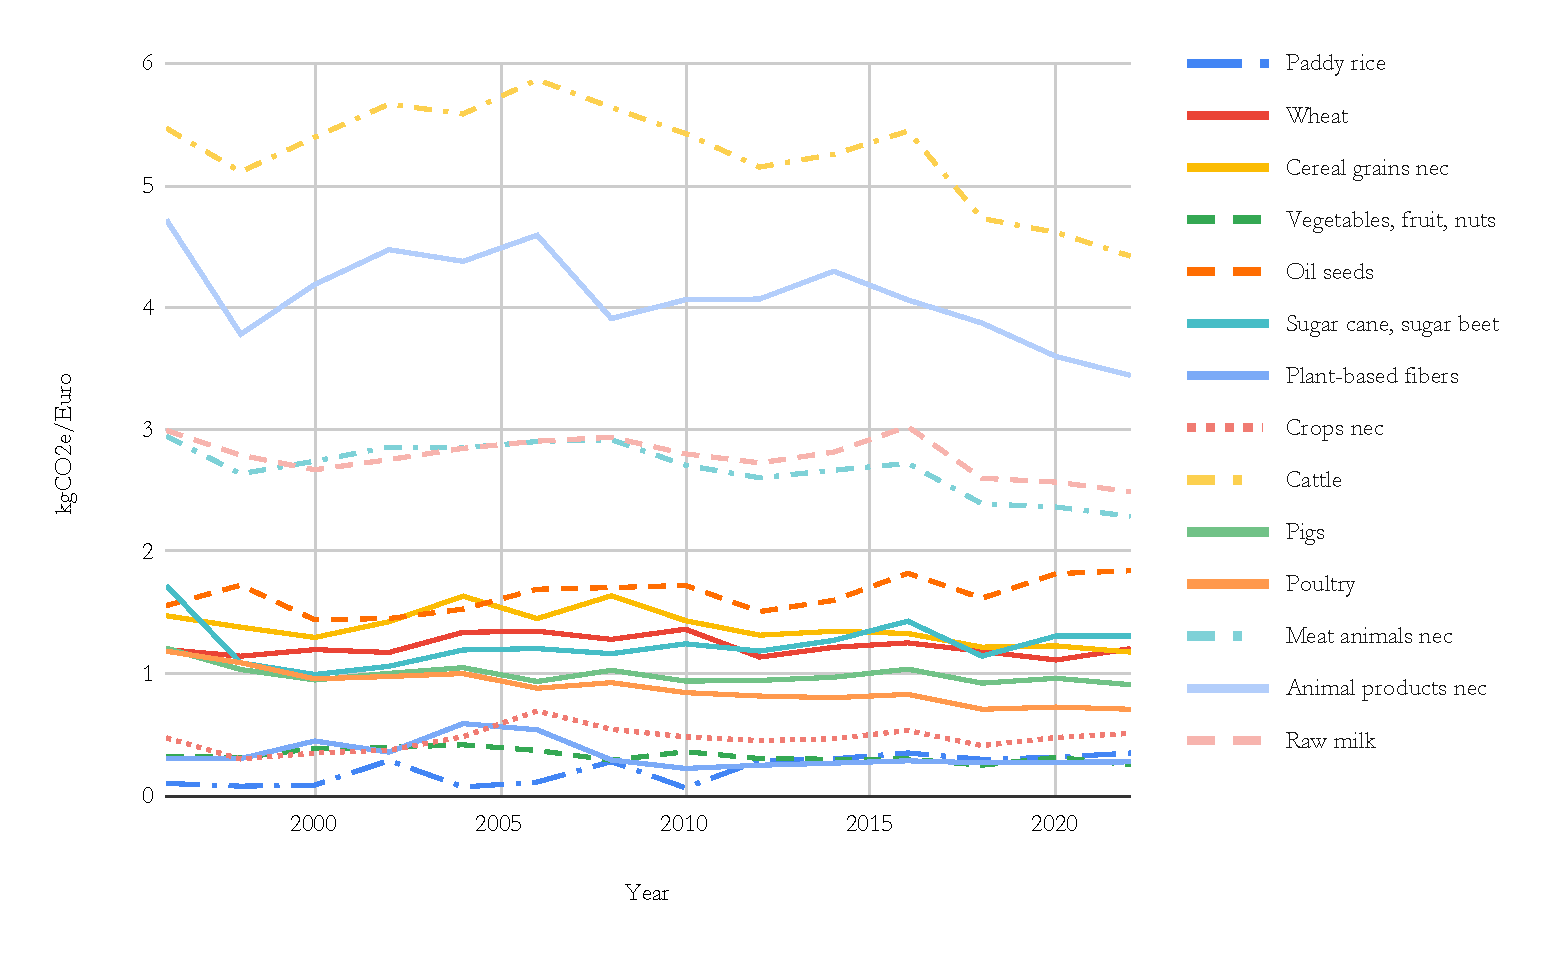
\includegraphics[width=0.9\textwidth]{inflated_adjusted}
\caption{The inflation-adjusted multipliers per sector for French agriculture 1996 - 2022}\label{fig:adjustedmultipliers} 
\end{figure}

In order to determine the trend in the evolution of the multipliers, the data was normalized relative to the starting year (1996) and the data for each sector was fit to a straight line. The slope of the line then gives us the averge percentwise change of the multipliers per year. Fig. \ref{fig:slope} shows the slopes of the normalized multipliers, ordered from smallest to largest. 

\begin{figure}[H]
\centering
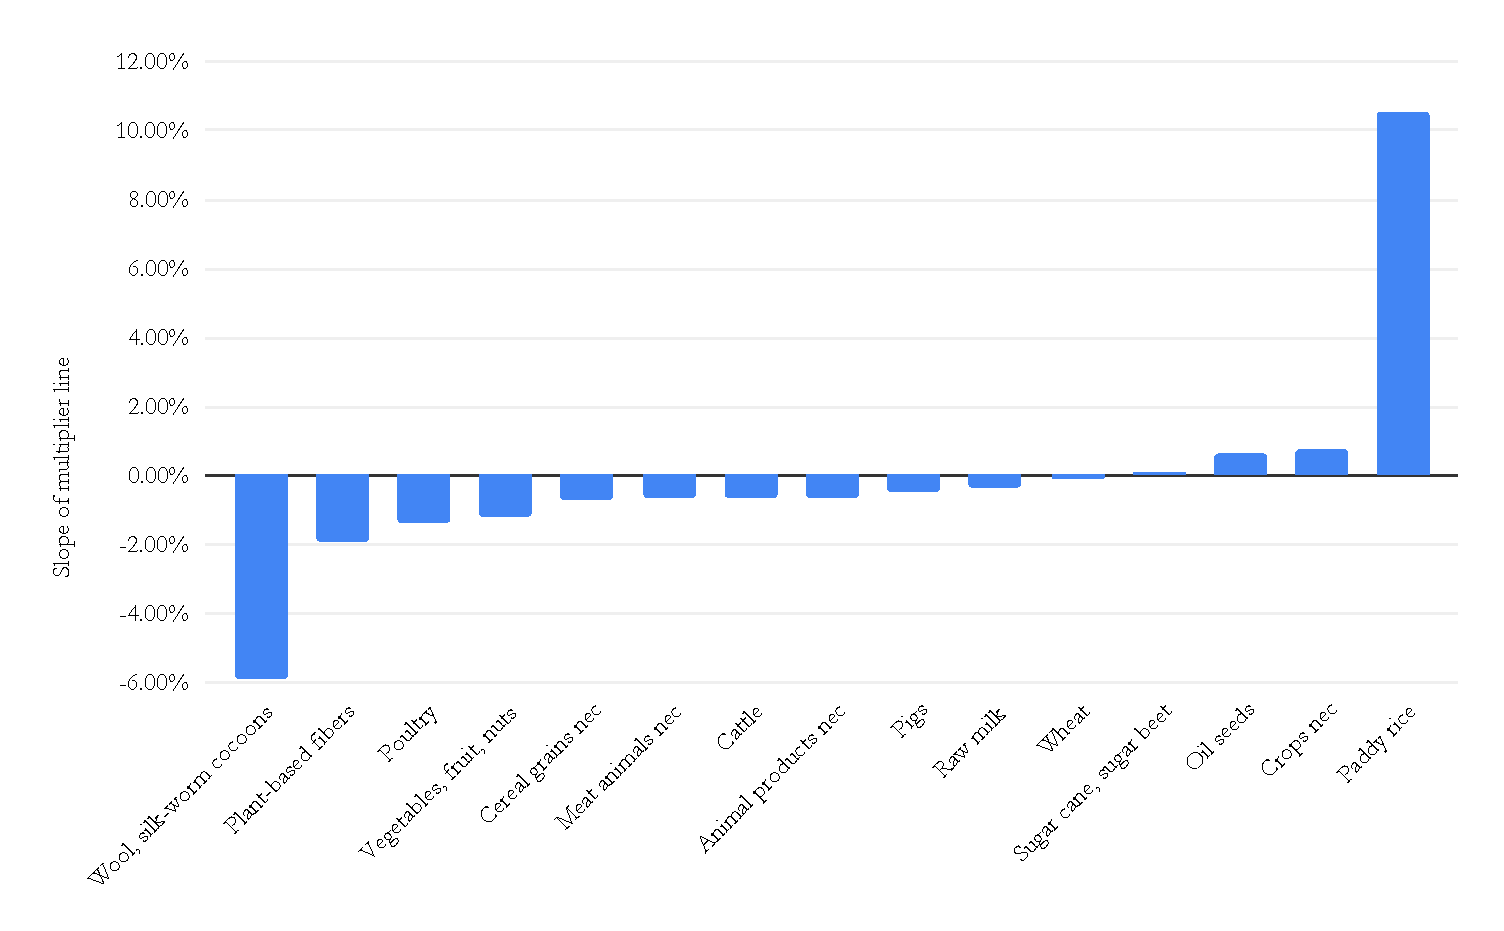
\includegraphics[width=0.9\textwidth]{slope}
\caption{The slope of the normalized multiplier line for each sector for the period 1996 - 2022}\label{fig:slope} 
\end{figure}

The average slope was -0.12\% per year, indicating that the multipliers are in fact trending very slightly downward. From Fig. \ref{fig:slope} it can be clearly seen that most slopes were less than -2\% per year. Outliers are the sectors "wool, silk-worm cocoons" and paddy rice. Wool trends strong negative, but this is mostly due to the erratic behavior of the multiplier, which exhibited a severe spike around 2008 before decrease towards 2022 and landed at essentially the same value as 1996. Paddy rice exhibits a strong increase of over 10\%, but has the lowest multiplier in terms of absolute value to begin with. The multipliers with the largest absolute value (cattle, raw milk, etc) exhibit the least amount of change.

In order to put the findings in context, we additionally calculated the total agricultural footprint by summing the total impacts for each of the sectors considered. Fig. \ref{fig:totalfootprint} shows the total footprint for agricultural sectors of France during the time periode considered. Despite some oscillations, the footprint is essentially stagnant or even slightly decreasing (see trendline in figure).

\begin{figure}[H]
\centering
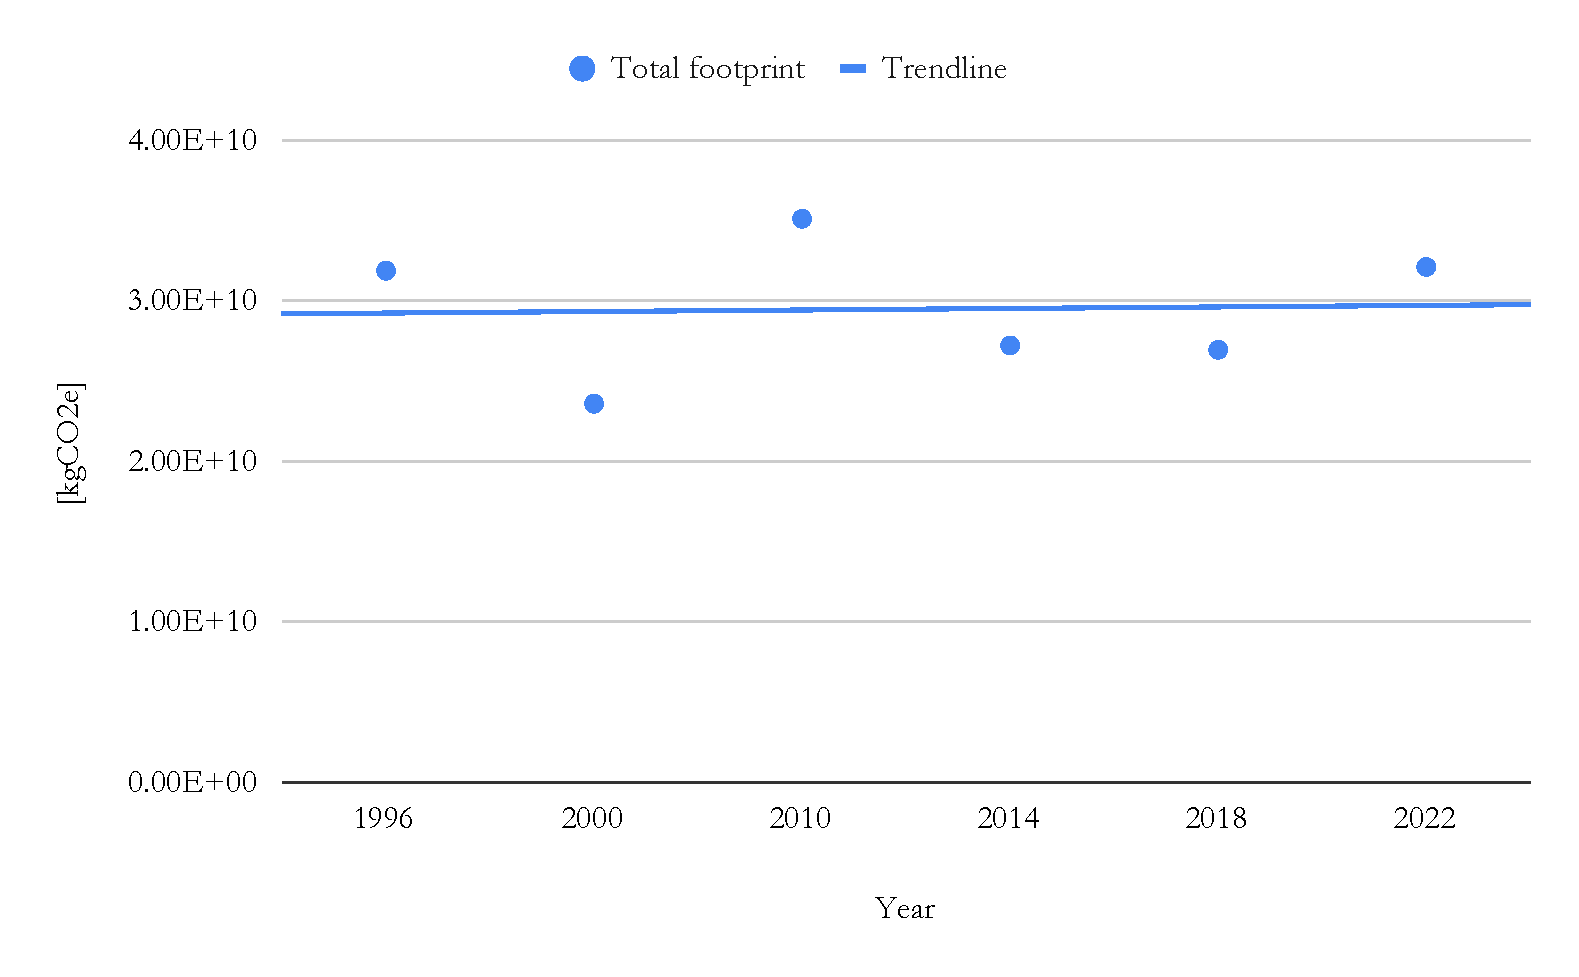
\includegraphics[width=0.9\textwidth]{totalfootprint}
\caption{The slope of the normalized multiplier line for each sector for the period 1996 - 2022}\label{fig:totalfootprint} 
\end{figure}

\section{Discussion}

Multipliers basically constant. Indicates no significant improvement in technology since 1996. (Discuss in context with energy article!)

Discuss uncertainty about findings due to simplification of inflation data.

France has reported a decrease in agriculture emissions. Since we are considering multipliers and these and the footprint are relatively stable this could indicate an increase in emissions import. 

Overall, when footprint is considered, Frances agricultural sector is not improving.

\bibliography{IOreport}

\appendix

\section{Python code}

\begin{lstlisting}

# %%
# Load Libraries
import pymrio
import numpy as np
import pandas as pd

# Define Inputs
Country = 'FR'
charact_table = pd.read_csv('public_char_factors.csv',  sep='\t')
ghg = 'GHG emissions (GWP100) | Problem oriented approach: baseline (CML, 2001) | GWP100 (IPCC, 2007)'

years = [str(year) for year in [*range(1996, 2024, 2)]]

# %%
# Next we iterate over the year range
for year in years:
  currentpath = 'IOT_'+year+'_pxp.zip'
  # Load data
  print('Loading data for ', year)
  current_exio = pymrio.parse_exiobase3(path=currentpath)
  # Calculate system
  print('Calculating data for ', year)
  current_exio.calc_all()
  # Characterize system
  print('Characterizing data for ', year)
  current_multiplier = current_exio.impacts.M[Country].loc[[ghg]].iloc[:, 0:15]
  # Store relevant multipliers
  current_multiplier.to_excel('multipliers'+year+'.xlsx')
  print('Calculation for year ', year, ' complete')
  
\end{lstlisting}

\end{document}